\documentclass{article}
\usepackage{tikz} 
\usetikzlibrary{shapes.misc,patterns,hobby}
\usepackage{pgfplots}
\usepgfplotslibrary{fillbetween}
%\usepackage[active,tightpage]{preview}  %generates a tightly fitting border around the work
%\PreviewEnvironment{tikzpicture}
%\setlength\PreviewBorder{2mm}
\usepackage{xcolor}
\definecolor{myred}{RGB}{196,19,47} 
\definecolor{myblue}{RGB}{0,139,139}

\pgfplotsset{
  /pgfplots/colormap={eugen}{%
    color(0cm) = (black!1);
    color(1cm) = (white!1);}
}

\begin{document}
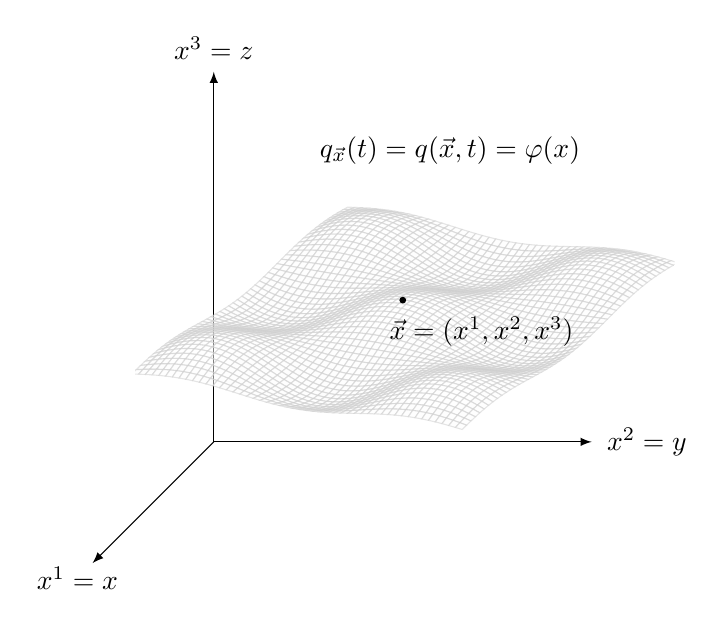
\begin{tikzpicture}[>=latex]

%Koordinatensystem (3D)
\draw[->, thin] (1,1.3,0) to (1,1.3,4);
\node at (1,1.3,4.5) {$x^1 = x$};
\draw[->, thin] (1,1.3,0) to (5.8,1.3,0);
\node at (6.5,1.3,0) {$x^2 = y$};
\draw[->, thin] (1,1.3,0) to (1,6,0);
\node at (1,6.3,0) {$x^3 = z$};
  
%Feld
\begin{axis}[xmin=-7,xmax=7,ymin=-5,ymax=5,zmin=-7,zmax=7,axis lines=none,colormap name=eugen,opacity=0.5]
 \addplot3[
   surf,
   shader=faceted,
   samples=50,
   domain=-2*pi:2*pi,
   y domain=-2*pi:2*pi
 ]{cos(0.7*deg(x))*cos(0.7*deg(y))};
\end{axis}


\filldraw (3.4,3.1) circle (1pt); 
\node at (4.4,2.7) {$\vec{x} = (x^1,x^2,x^3)$};

\node at (4,5) {$q_{\vec{x}}(t) = q(\vec{x},t) = \varphi(x)$};

\end{tikzpicture}
\end{document}